\chapter{Introduction}\label{C:intro}
Software is embedded into our daily lives. From ensuring that a plane remains airborne to helping doctors administer treatment. With these critical systems, testing is needed to ensure functional correctness and error free usage. Without correct testing \todo{Should I explain what is 'correct testing'?}, incidents can occur resulting in serious injury and death. A notable example is the Therac-25 where patients were dosed with sometimes thousands of times the greater than normal amount of radiation resulting in several deaths \cite{therac}.

\section{Motivation}
How can we ensure a change has not broken the system ? A suite of tests is run on a project in an attempt to cover the majority of situations. The number of situations is often endless, so covering the majority of situations can incur a large number of tests and in turn take several hours to run. All this for potentially one change. The idea of test cases is becoming an increasing concern within software development areas. Driven by agile methodologies incorporating practices like test driven development and continuous integration.
\todo{Link this better ?}
Test cases are added throughout a project, often when either a piece of code is altered, new code is developed or a bug gets fixed. With test cases being added throughout, how can we ensure that the first test case is not doing the same as the thousandth.

\section{Approach}

During a tests execution, it leaves a 'paper trail' behind. This trail is the method executions that are called during the test, referred to as the tests spectrum. In figure \ref{fig:spectrum} we see the spectrum's of four different tests. A spectrum will be the set of data that will be analysed using different algorithms to determine how related a test is with another.

\begin{figure}[h]
\caption{Test Spectrum}
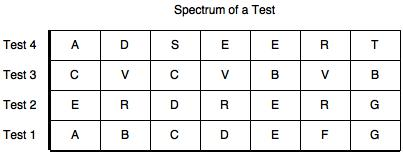
\includegraphics[]{Spectrum.jpg}
\label{fig:spectrum}
\end{figure}

\section{Aim}

The aim of the project is to identify different approaches that give the developers an idea on the number of redundant test cases that are contained within a project. It should allow the developer to run a set of pipelines they specify and view the results on a GUI, allowing manual inspection to determine if they are truly redundant. This means that the tool is useful for gaining an overview and understanding of the condition of the current test suite. A potential use of the tool is to allow for splitting of the somewhat redundant tests into separate test suites and during the life cycle, the seperate test suites can be run at different times. For example, during continuous integration, one test suite can be run, and the other over night. Ensuring that we are not losing any probability of finding a bug, instead redistributing the test time.

\section{How to trace a test}
\todo{Should this be in the background or introduction?}
Dr David Pearce is currently writing a language called Whiley, which contains an extended static checking framework in order to eliminate run time exceptions through formal verification techniques. This language is written in Java as such it was the language chosen to perform the tracing. There are two viable approaches, AspectJ or Java Debugging Interface (JDI). JDI is similar to using a observer pattern, when a set of classes methods are called, the listening classes will be notified. AspectJ utilises byte code weaving; where an aspect is adding behaviour to existing code without modifying the code itself. It uses a point cut to identify what code is weaved and where in the code \cite{aspectwiki}. AspectJ allows for several methods to achieve tracing through byte code weaving:

\begin{itemize}
\item Compile time:
The classes are compiled with the aspect weaved into them. So that when the jar is executed, the methods have the byte code from the aspect weaved into it already \cite{weaving}.
\item Load time:
This involves binary weaving deferred until the point in which a class loader will attempt to load in a class file and define it to the java virtual machine (JVM) \cite{weaving}.
\end{itemize}

Load time weaving was the preferred method. The projects often had a large number of modules and dependencies. If compile time weaving was to be used, then each would have to be re-compiled using the AspectJ's compiler. Instead, load time allows for easier integration with existing projects to trace.

Between JDI and AspectJ, AspectJ allows for stronger ability to choose which methods to record and gives more ability to retrieve the parameters however JDI was faster to execute. The decision to use AspectJ was based off a trade off between more information and performance. The analysis framework was able to be altered to increase the performance of it, so having the extra information that AspectJ gave was more important than an taking less time to execute.